%
% bewegung.tex -- Begründet die Bewegung von Wirbelringen
%
% !TEX root = ../../buch.tex
% !TEX encoding = UTF-8
%
\section{Bewegung eines Wirbelrings\label{Wirbelringe:Bewegung}}
\kopfrechts{Bewegung eines Wirbelrings}%
Bisher wurde die Bewegung eines Wirbelrings noch nicht weiter betrachtet. 
Doch wie man bereits bei Rauchringen beobachten kann, bleiben diese nicht an einem Ort stehen, sondern bewegen sich. 
Um diese Verhalten zu begründen, wird das Biot-Savart-Gesetz \cite{Wirbelringe:FuehrerdurchdieStroemungslehre} im folgenden Abschnitt angewandt.

\subsection{Biot-Savart-Gesetz}

Das Biot-Savart-Gesetz
\index{Biot-Savart-Gesetz}%
\[
d \vec{B}
=
\frac{\mu_0}{4\pi}\frac{I \,d \vec{l} \times \vec{r}}{\lvert \vec{r}^{\,3}\rvert }
\]  % Note : diese Definition weicht von der Definiton 3.2 im ELT2 Skript ab da dort ein Richtungsvektor verwendet wird -> ein r (dort ein R) kürzt sich heraus
wird typischerweise in der Elektrotechnik angewandt, um das Magnetfeld von bewegten Ladungen zu beschreiben (hier nur auf einen Strom durch einen Leiter vereinfacht).
Es kann nur bei geschlossenen Stromkreisen verwendet werden. 

Damit wir das Gesetz nutzen können, müssen wir zunächst die Grössen anpassen und überprüfen, ob das überhaupt erlaubt ist. 
Die elektrodynamischen Grössen haben jeweils ein Gegenstück in der Strömungsmechanik:

\begin{center}
    \begin{tabular}{lcl}
    stromdurchflossener Leiter          & \(\Leftrightarrow \) & Wirbelfaden \\
    Stromstärke \(I\)                   & \(\Leftrightarrow \) & Zirkulation \(\Gamma\) \\
    Stromdichtevektor \(\vec{\jmath}\)       & \(\Leftrightarrow \) & Wirbelstärkevektor \(\vec{\omega}\)\\
    magnetische Feldstärke \(\vec{H}\)  & \(\Leftrightarrow \) & Geschwindigkeit \(\vec{u}\) \\
    \end{tabular}
\end{center}

Im Folgenden wird der Wirbelstärkevektor nicht verwendet.
Jedoch ist der Zusammenhang vom Wirbelstärkevektor zum Stromdichtevektor etwas intuitiver als die Zirkulation zur Stromstärke.

Die Maxwellgleichungen (siehe Abschnitt \ref{chapter:maxwell}) sehen vor, dass das \(\vec{B}\)-Feld quellenfrei ist. 
Da wir nur inkompressible Fluide betrachten, ist dies gegeben.

Setzt man nun die entsprechenden Grössen in das Biot-Savart-Gesetz
\[
d\vec{u}
=
\frac{\Gamma}{4\pi}\frac{d\vec{l} \times \vec{r}}{\lvert \vec{r}^{\,3}\rvert }
\]
ein, lässt sich damit die Geschwindigkeitsänderung eines Punktes durch ein Wirbelfadenelement beschreiben.
Um die Rechnung zu vereinfachen, können wir annehmen, dass der Wirbelfaden  dünn ist im Vergleich zum Durchmesser des Rings aus der Wirbellinie.
Mit dem Integral
\begin{equation}
    \label{Wirbelringe:eq:WirbelSpeed}
    \vec{u}
    =
    \int_{\text{Wirbellinie}} \frac{\Gamma}{4\pi}\frac{d\vec{l} \times \vec{r}}{\lvert \vec{r}^{\,3}\rvert}
\end{equation}
über diesen Wirbelfaden
erhalten wir die induzierte Geschwindigkeit, welche durch den Wirbelfaden entsteht.
Da dieses Gesetz aus der Elektrotechnik stammt, spricht man in der Strömungsmechanik von einer induzierten Geschwindigkeit.
\index{induzierte Geschwindigkeit}%
\index{Geschwindigkeit, induziert}%

Um die selbstinduzierte Geschwindigkeit zu berechnen, wählen wir einen in der \(x\)-\(y\)-Ebene liegenden Wirbelring mit Radius \(a\).
Wie bereits erwähnt ist der Radius des Wirbelfadens vernachlässigbar klein.
Uns interessiert irgendein Punkt, der auf der Wirbellinie liegt.
Somit ist
\[
\vec{r} = 
\begin{pmatrix}
    a \cos \varphi\\
    a \sin \varphi\\
    0    
\end{pmatrix}
\qquad
\text{und}
\qquad
d\vec{l} = 
\begin{pmatrix}
    -a \sin \varphi\\
    a \cos \varphi\\
    0    
\end{pmatrix}
\,d\varphi .
\] 
Setzt man diese in Gleichung \eqref{Wirbelringe:eq:WirbelSpeed} ein und löst das Kreuzprodukt 
\[
d\vec{l}\times\vec{r} 
= 
\begin{pmatrix}
    -a \sin \varphi\\
    a \cos \varphi\\
    0
\end{pmatrix}
\times
\begin{pmatrix}
    a \cos \varphi\\
    a \sin \varphi\\
    0    
\end{pmatrix}
=
\begin{pmatrix}
    0\\
    0\\
    a^2
\end{pmatrix}
\]
auf, erhält man nach Einsetzen der Integrationsgrenzen von 0 bis \(2\pi\)
\begin{align*}
\vec{u}
&=
\int_{0}^{2\pi} \frac{\Gamma}{4\pi}\frac{1}{a^3}
\begin{pmatrix}
    0\\
    0\\
    a^2
\end{pmatrix}
\,d\varphi\\
&=\frac{\Gamma}{2a^3}
\begin{pmatrix}
    0\\
    0\\
    a^2
\end{pmatrix}\\
&=\frac{\Gamma}{2a}\hat{e}_z.
\end{align*}    
Dies deckt sich auch mit der Annahme, dass der Kreisumfang und der Radius immer senkrecht zueinander stehen.
Zusätzlich ist ersichtlich, dass mit zunehmender Grösse des Wirbelrings die Geschwindigkeit des Wirbelrings abnimmt.

Würde man dieselbe Rechnung für einen geraden Wirbelfaden durchführen, würde auffallen, dass das Ergebnis für Punkte auf der Wirbellinie null ist.
Aufgrund der Symmetrie kann der Wirbelfaden auf sich selbst keine Geschwindigkeit induzieren.
Damit sich ein Wirbelfaden von sich aus bewegt, muss dieser zumindest ein wenig gekrümmt sein.
Ein zweiter Wirbelfaden würde auch zu einer induzierten Geschwindigkeit führen. 
Dies betrachten wir hier aber nicht weiter. 

\subsection{Bewegung eines Teilchens}

\begin{figure}
\centering
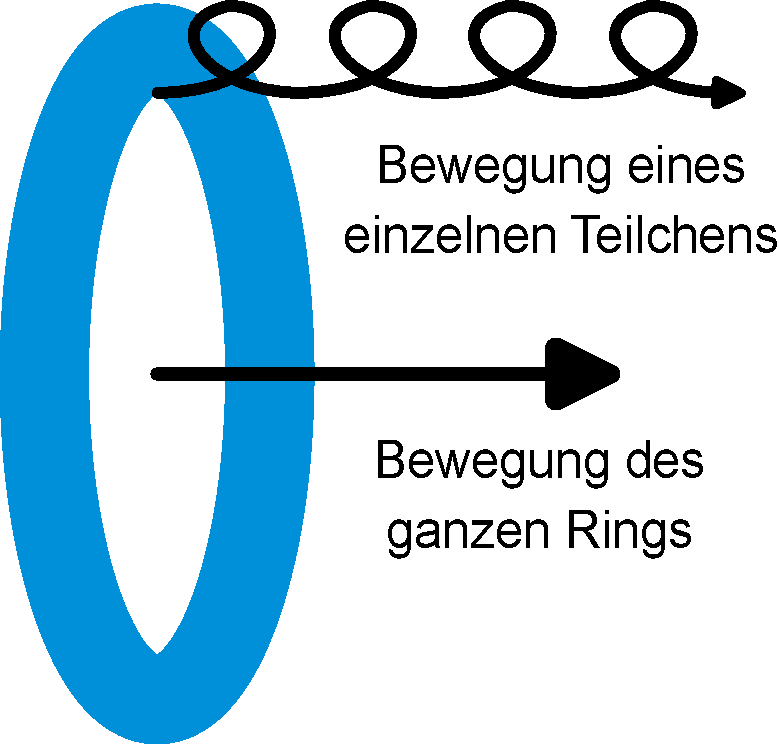
\includegraphics[width=0.4\textwidth]{papers/wirbelringe/fig/ausbreitung_teilchen.pdf}
\caption{Bewegung eines einzelnen Teilchen ToDo besseri Farb für de Ring??? \label{buch:papers:Wirbelringe:fig:ausbreitung_teilchen}}
\end{figure}

Eine interessante Kurve zeichnet sich ab, wenn man ein einzelnes Teilchen beobachtet.
Es bildet sich eine Zykloide.
\index{Zykloide}%
Die Grösse der Zykloide hängt von der Höhe der Zirkulation ab.
Dies ist in Abbildung \ref{Wirbelringe:fig:ausbreitung_teilchen} dargestellt.
